
In this section, we give a brief overview of the LTE-U, 
introduce the coexistence issues and set the scene for the subsequent in-depth study of each of them. 

\subsection{LTE-U Overview}

LTE-U leverages channel bonding techniques of LTE to transmit downlink data in unlicensed 5 GHz channels. The control channel and latency sensitive downlink data are transmitted over a licensed channel and the rest of the data over the unlicensed one. 

Unlike Wi-Fi where listen-before-talk (LBT) is a fundamental MAC mechanism in the CSMA protocol, LTE-U does not sense the medium before transmitting. Instead, it continuously transmits downlink data during an ON period $T_{ON}$, followed by an idle OFF period $T_{OFF}$. The fraction of the time spent in the ON periods is called a duty cycle, i.e. $\eta = T_{ON} / (T_{ON} + T_{OFF})$. 


To share fairly with Wi-Fi, LTE-U must have an adaptive duty cycle. 
Each LTE-U access point should continuously monitor the traffic in the environment, 
estimate the medium utilization statistics and 
adjust the duty cycle accordingly. The exact duty cycle adaptation algorithm is not specified in the LTE-U standard, and the only such scheme available at the moment is the one proposed by Qualcomm called CSAT~\cite{lteuforum_csat}, further explained in Section~\ref{sec:csatdef}.


\begin{figure}[!ht]
 \centering
    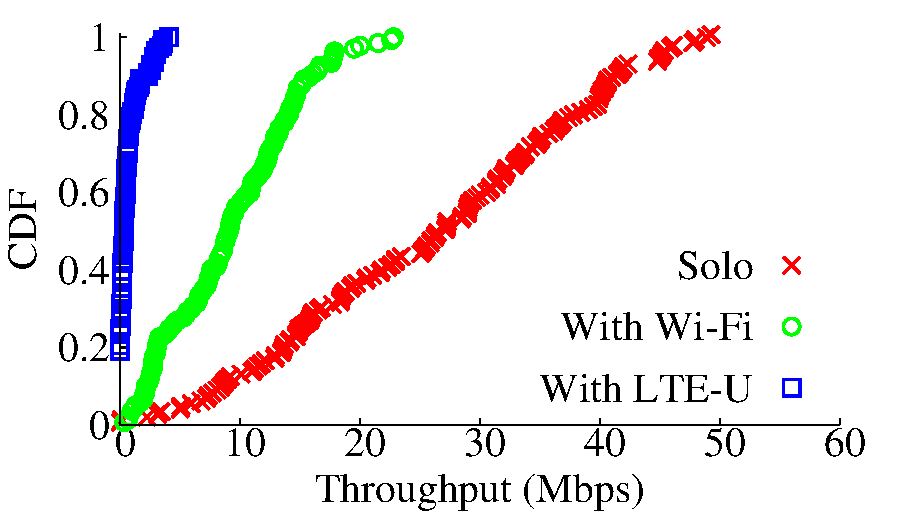
\includegraphics[width=2.8in]{./figures/motivation}
 \caption{LTE-U in a lab: Wi-Fi with no added APs (Solo), with interfering Wi-Fi AP, and with interfering LTE-U AP.}
  \label{fig:lteu_lab}
\end{figure}



\subsection{LTE-U Impact in the Wild}

We start by illustrating the effect LTE-U can have on an existing Wi-Fi deployment. We connect a laptop $L$ to an existing Wi-Fi access point in a lab and use iperf to generate a saturated TCP connection. The floorplan is depicted in Figure~\ref{fig:lteu_lab}. We walk all over the coverage area (denoted with the red line) of the access point and measure the observed TCP throughput. 

We then place a second access point and a second client in the vicinity of the previous deployment, and we run a fully backlogged UDP traffic between them, over the same Wi-Fi channel. We plot the TCP throughput of laptop $L$ in green (With Wi-Fi). As expected, the throughput has dropped by approximately half, because the two Wi-Fi links share the same medium. 

Finally, we remove the second access point and place an LTE-U node instead, running CSAT, and we plot the TCP throughput of laptop $L$ in blue (With LTE-U). As can be seen, the throughput has dropped significantly, with the median TCP throughput dropping by almost 10 times!
We observe similar effects in other experiments that we perform in public places, such as cafes, as discussed in Section~\ref{sec:eval}.



\subsection{Why LTE-U Chokes Wi-Fi?}

%{\bf BR: Why do we see throughput decrease in this particular case?}

There are several reasons why LTE-U severely affects Wi-Fi. The two issues widely discussed in existing literatures are around LTE-U's use of energy detection and Wi-Fi rate adaptation (c.f. \cite{google, cablelabs}). 

In this paper we focus on the issue of the utilization-based duty cycle adaptation, which to the best of our knowledge hasn't been studied before. 
According to CSAT~\cite{lteuforum_csat}, LTE-U increases its duty cycle until the observed Wi-Fi's medium utilization reaches a threshold. 
The implicit assumption is that a backlogged Wi-Fi link will have high medium utilization. While this may be true in small test-beds, it doesn't hold in the real world where many neighbouring links can prevent a backlogged link from achieving high utilization. An LTE-U base-station may not observe all these links, and can wrongfully conclude that Wi-Fi is not backlogged because medium is idle, leading to duty cycle increases and eventual Wi-Fi starvation.


%The first one is that LTE-U only detects Wi-Fi using energy detection, with a threshold of -62 dBm. Typical Wi-Fi noise floor is around -82 dBm so an LTE-U node can create as much as 20 dB of interference over the noise floor without realizing it, which is clearly detrimental for Wi-Fi. The second issue is the effect of the collisions induced by LTE-U on Wi-Fi's rate adaptation. Without listen-before-talk (LBT), LTE-U transmissions will inevitably collide with progressing Wi-Fi frames. Given that collisions are rare in Wi-Fi networks with LBT, most rate adaptation algorithms will misinterpret such frame losses as bad channel conditions, resulting in Wi-Fi reducing its own transmission rate and throttling its own throughput. This phenomenon will affect a large number of already deployed Wi-Fi access points. To mitigate this, we propose a solution based on CTS-to-self mechanism that sends the correct signal back to Wi-Fi and mitigates these effects.


\nop{
For each of these observed coexistence issues between LTE-U and Wi-Fi, we have done thorough analysis with experimental validations (Section~\ref{sec:csat} and ~\ref{sec:sensing}). 
For each of them we propose a novel remedy that addresses the observed issue. 
However, our study (Section~\ref{sec:ineff}) further shows that in some scenarios LTE-U has a fundamental deficiency, where the absence of LBT reduces spectral efficiency as it causes more collisions than necessary. 
}



\subsection{Fairness}
\label{sec:fairness}

At a high level, the Wi-Fi and LTE-U coexistence problem is about CSMA and TDMA coexisting in the same spectrum. The two approaches have fundamentally different properties. On the one hand, Wi-Fi senses the carrier and reacts on any on-air transmission. It is more reactive, potentially offering more opportunities for statistical multiplexing. At the same time, Wi-Fi MAC is known to be inefficient in several scenarios (hidden terminal, exposed terminal). On the other hand, TDMA is less reactive and adjusts its duty cycle based on average medium utilization. It is therefore not entirely clear how to define fair coexistence in a setting where two technologies share the same spectrum. 

LTE-U specification offers a very limited definition of fairness with Wi-Fi devices sharing the same channel~\cite{lteuforum_lteu}. It considers only two criteria. 
The first one is that an LTE-U AP shouldn't set its duty cycle to more than 50\% in the presence of a single fully backlogged Wi-Fi AP.
The second one is that it shouldn't set its duty cycle to more than 33\% in presence of two fully backlogged Wi-Fi AP.
No coexistence guarantees are offered for any other network scenario.

To generalize fairness across all scenarios, we use a more general definition of fairness, also suggested by Wi-Fi Alliance~\cite{wifialliance}.
We say that an LTE-U algorithm is {\em fair} to Wi-Fi if a deployed instance of LTE-U in an unlicensed channel affects Wi-Fi users in the channel no worse than the impact that would result from an additional Wi-Fi device or Wi-Fi network introduced into the channel supporting the same traffic load as the system. 

Finally, we note that in this paper we focus on throughput as our primary metric, since a user with very low throughput will perceive the network as disconnected. However, we note that there are many other important metrics which also need to be considered, such as latency and energy consumption (c.f. \cite{google, cablelabs}). We leave these as future work. 



